% AdaScale: Cache-Aware Parallel AdaEvolve — Conference Poster
% Self-contained: no external theme files required
% Compile with: pdflatex poster.tex

\documentclass[final]{beamer}

\usepackage[T1]{fontenc}
\usepackage{lmodern}
\usepackage[size=custom,width=120,height=72,scale=1.0]{beamerposter}
\usepackage{graphicx}
\usepackage{booktabs}
\usepackage{tikz}
\usetikzlibrary{positioning,arrows.meta}
\usepackage{amsmath}
\usepackage{xcolor}
\usepackage{ragged2e}

% ====================
% Colours
% ====================
\definecolor{berkeleyblue}{RGB}{0,50,98}
\definecolor{berkeleygold}{RGB}{253,181,21}
\definecolor{blockbg}{RGB}{245,248,252}
\definecolor{alertbg}{RGB}{255,249,215}

\usetheme{default}
\setbeamercolor{background canvas}{bg=white}
\setbeamertemplate{navigation symbols}{}

% ====================
% Layout lengths
% ====================
\newlength{\sepwidth}
\newlength{\colwidth}
\setlength{\sepwidth}{0.025\paperwidth}
\setlength{\colwidth}{0.3\paperwidth}
\newcommand{\separatorcolumn}{\begin{column}{\sepwidth}\end{column}}

\newlength{\hdrh}
\setlength{\hdrh}{10.5cm}

% ====================
% Block environments
% ====================
\newenvironment{posterblock}[1]{%
  \noindent\begin{minipage}[t]{\colwidth}%
    \noindent\colorbox{berkeleyblue}{%
      \begin{minipage}[t]{\dimexpr\colwidth-2\fboxsep\relax}%
        \vspace{3pt}\color{white}\large\bfseries #1\vspace{3pt}%
      \end{minipage}}\\[-1pt]%
    \noindent\colorbox{blockbg}{%
      \begin{minipage}[t]{\dimexpr\colwidth-2\fboxsep\relax}%
        \vspace{6pt}\RaggedRight\small%
}{%
        \vspace{6pt}%
      \end{minipage}}%
  \end{minipage}\par\vspace{8pt}%
}

\newenvironment{posteralert}[1]{%
  \noindent\begin{minipage}[t]{\colwidth}%
    \noindent\colorbox{berkeleygold}{%
      \begin{minipage}[t]{\dimexpr\colwidth-2\fboxsep\relax}%
        \vspace{3pt}\color{berkeleyblue}\large\bfseries #1\vspace{3pt}%
      \end{minipage}}\\[-1pt]%
    \noindent\colorbox{alertbg}{%
      \begin{minipage}[t]{\dimexpr\colwidth-2\fboxsep\relax}%
        \vspace{6pt}\RaggedRight\small%
}{%
        \vspace{6pt}%
      \end{minipage}}%
  \end{minipage}\par\vspace{8pt}%
}

\newcommand{\heading}[1]{%
  \vspace{3pt}\noindent{\small\bfseries\color{berkeleyblue}#1}\par\vspace{1pt}}

% ====================
% Prompt diagram (replaces the broken tikzpicture)
% Uses \linewidth so it always fills the block width cleanly.
% ====================
\newcommand{\promptdiagram}{%
  \vspace{4pt}%
  % Row 1: coloured boxes
  \noindent
  \colorbox{berkeleyblue!15}{%
    \begin{minipage}[c][1.4em]{0.70\linewidth}%
      \centering\small system message ($\sim$3500 tokens, \textit{stable})%
    \end{minipage}}%
  \colorbox{berkeleygold!45}{%
    \begin{minipage}[c][1.4em]{\dimexpr0.30\linewidth-2\fboxsep\relax}%
      \centering\small parent + state%
    \end{minipage}}%
  % Row 2: captions underneath each box
  \par\vspace{1pt}%
  \noindent
  \begin{minipage}[t]{0.70\linewidth}%
    \centering\scriptsize\color{black!60}
    evaluator code, framework instructions%
  \end{minipage}%
  \begin{minipage}[t]{0.30\linewidth}%
    \centering\scriptsize\color{black!60}
    $\sim$500 tokens, churns%
  \end{minipage}%
  \vspace{4pt}%
}

% ====================
% Header
% ====================
\setbeamertemplate{headline}{%
  \begin{beamercolorbox}[wd=\paperwidth]{headline}%
    \begin{tikzpicture}%
      \fill[berkeleyblue] (0,0) rectangle (\paperwidth,\hdrh);
      \fill[berkeleygold] (0,0) rectangle (\paperwidth,0.45cm);
      \node[anchor=north, text=white,
            font=\fontsize{52}{58}\selectfont\bfseries, align=center]
        at (\paperwidth/2, \hdrh-0.3cm)
        {AdaScale:  Cache-Aware Parallel AdaEvolve};
      \node[anchor=north, text=white!88, font=\Large, align=center]
        at (\paperwidth/2, \hdrh-2.55cm)
        {Systems optimizations for adaptive LLM-guided evolutionary search};
      \node[anchor=north, text=white, font=\large, align=center]
        at (\paperwidth/2, \hdrh-4.35cm)
        {Mert Cemri \quad Matteo Guarrera \quad Elizabeth Polito
         \quad Dongwei Lyu \quad Sultan Daniels \quad Eric Xu};
      \node[anchor=north, text=berkeleygold, font=\normalsize\itshape, align=center]
        at (\paperwidth/2, \hdrh-6.05cm)
        {CS 294: Scalable AI Systems,\ Spring 2026 \quad---\quad UC Berkeley};
    \end{tikzpicture}%
  \end{beamercolorbox}%
}

% ====================
% Footer
% ====================
\setbeamertemplate{footline}{%
  \begin{beamercolorbox}[wd=\paperwidth]{footline}%
    \begin{tikzpicture}
      \fill[berkeleyblue] (0,0) rectangle (\paperwidth,1.3cm);
      \node[anchor=west, text=white, font=\normalsize, inner xsep=2cm]
        at (0,0.65cm) {CS 294: Scalable AI Systems};
      \node[anchor=east, text=white, font=\normalsize, inner xsep=2cm]
        at (\paperwidth,0.65cm) {Spring 2026};
    \end{tikzpicture}%
    \vspace{1.3cm}%
  \end{beamercolorbox}%
}

% ====================
\begin{document}
\begin{frame}[t]
\vspace{0.4cm}
\begin{columns}[t]
\separatorcolumn

% ============================================================
%  COLUMN 1
% ============================================================
\begin{column}{\colwidth}

\begin{posterblock}{Background}
  \textbf{SkyDiscover} is a framework for LLM-guided code discovery.
  \textbf{AdaEvolve} is one of its search algorithms: at each iteration
  it samples a parent program, asks an LLM to mutate it, evaluates the
  result, and updates a population of programs.

  \vspace{0.4em}
  AdaEvolve runs three nested adaptive control loops:

  \vspace{0.3em}
  \begin{center}
  \begin{tikzpicture}[
    lev/.style={draw=berkeleyblue!55, rounded corners=3pt, align=center,
                minimum width=26mm, minimum height=11mm, font=\small,
                fill=berkeleyblue!8},
    arr/.style={-{Latex[length=2mm]}, thick, berkeleyblue!45}]
    \node[lev] (l1) {\textbf{Per-island}\\\scriptsize adapt intensity};
    \node[lev, right=5mm of l1] (l2) {\textbf{Cross-island}\\\scriptsize UCB budget};
    \node[lev, right=5mm of l2] (l3) {\textbf{Meta}\\\scriptsize new paradigms};
    \draw[arr] (l1) -- (l2);  \draw[arr] (l2) -- (l3);
    \node[below=0.5mm of l1, font=\scriptsize, text=black!50] {per iter};
    \node[below=0.5mm of l2, font=\scriptsize, text=black!50] {across iters};
    \node[below=0.5mm of l3, font=\scriptsize, text=black!50] {on stagnation};
  \end{tikzpicture}
  \end{center}

  \vspace{0.2em}
  Our changes do \emph{not} touch this logic — we only restructure how
  LLM calls inside each iteration are issued.
\end{posterblock}

\begin{posteralert}{The Problem: Wasted Prefix Cache}
  A typical AdaEvolve prompt has a large \emph{static} prefix and a
  small \emph{dynamic} suffix:

  \promptdiagram

  vLLM hashes 16-token blocks with a chained SHA-256:
  \(h_i = \mathrm{SHA256}(h_{i-1} \,\Vert\, \text{tokens}_i)\).
  A single edit at position $k$ invalidates every block
  $\geq\!\lceil k/16\rceil$. Because the parent code changes every
  iteration, the chain breaks mid-prompt.

  \vspace{0.3em}
  \textbf{Measured cache hit rate: only 17\%.}
\end{posteralert}

\begin{posterblock}{Per-Iteration Cache Behavior}
  \begin{figure}
    \centering
    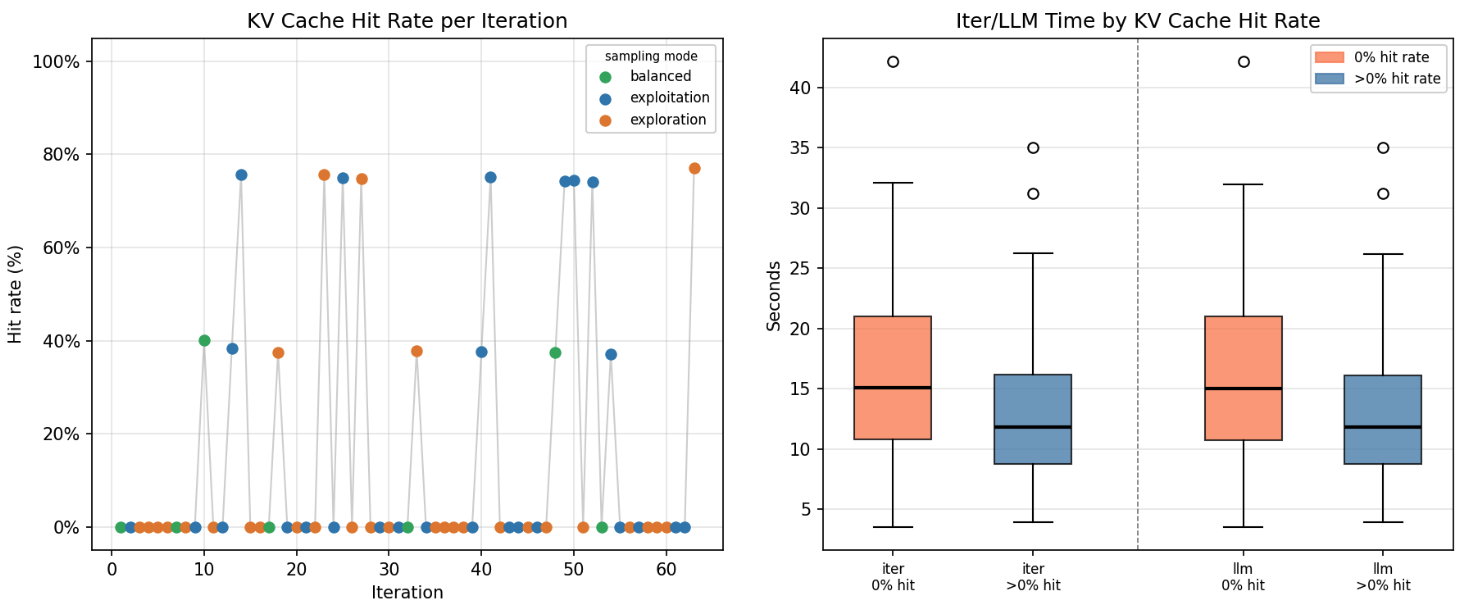
\includegraphics[width=0.96\textwidth]{figs/kv_cache_per_iter_motivation.png}
    \caption{\small Most iterations hit 0\% of the cache (left). Any
             non-zero hit removes $\sim$3\,s from the iteration (right).}
  \end{figure}
\end{posterblock}

\end{column}
\separatorcolumn

% ============================================================
%  COLUMN 2
% ============================================================
\begin{column}{\colwidth}

\begin{posterblock}{AdaEvolve Overview}
  \begin{figure}
    \centering
    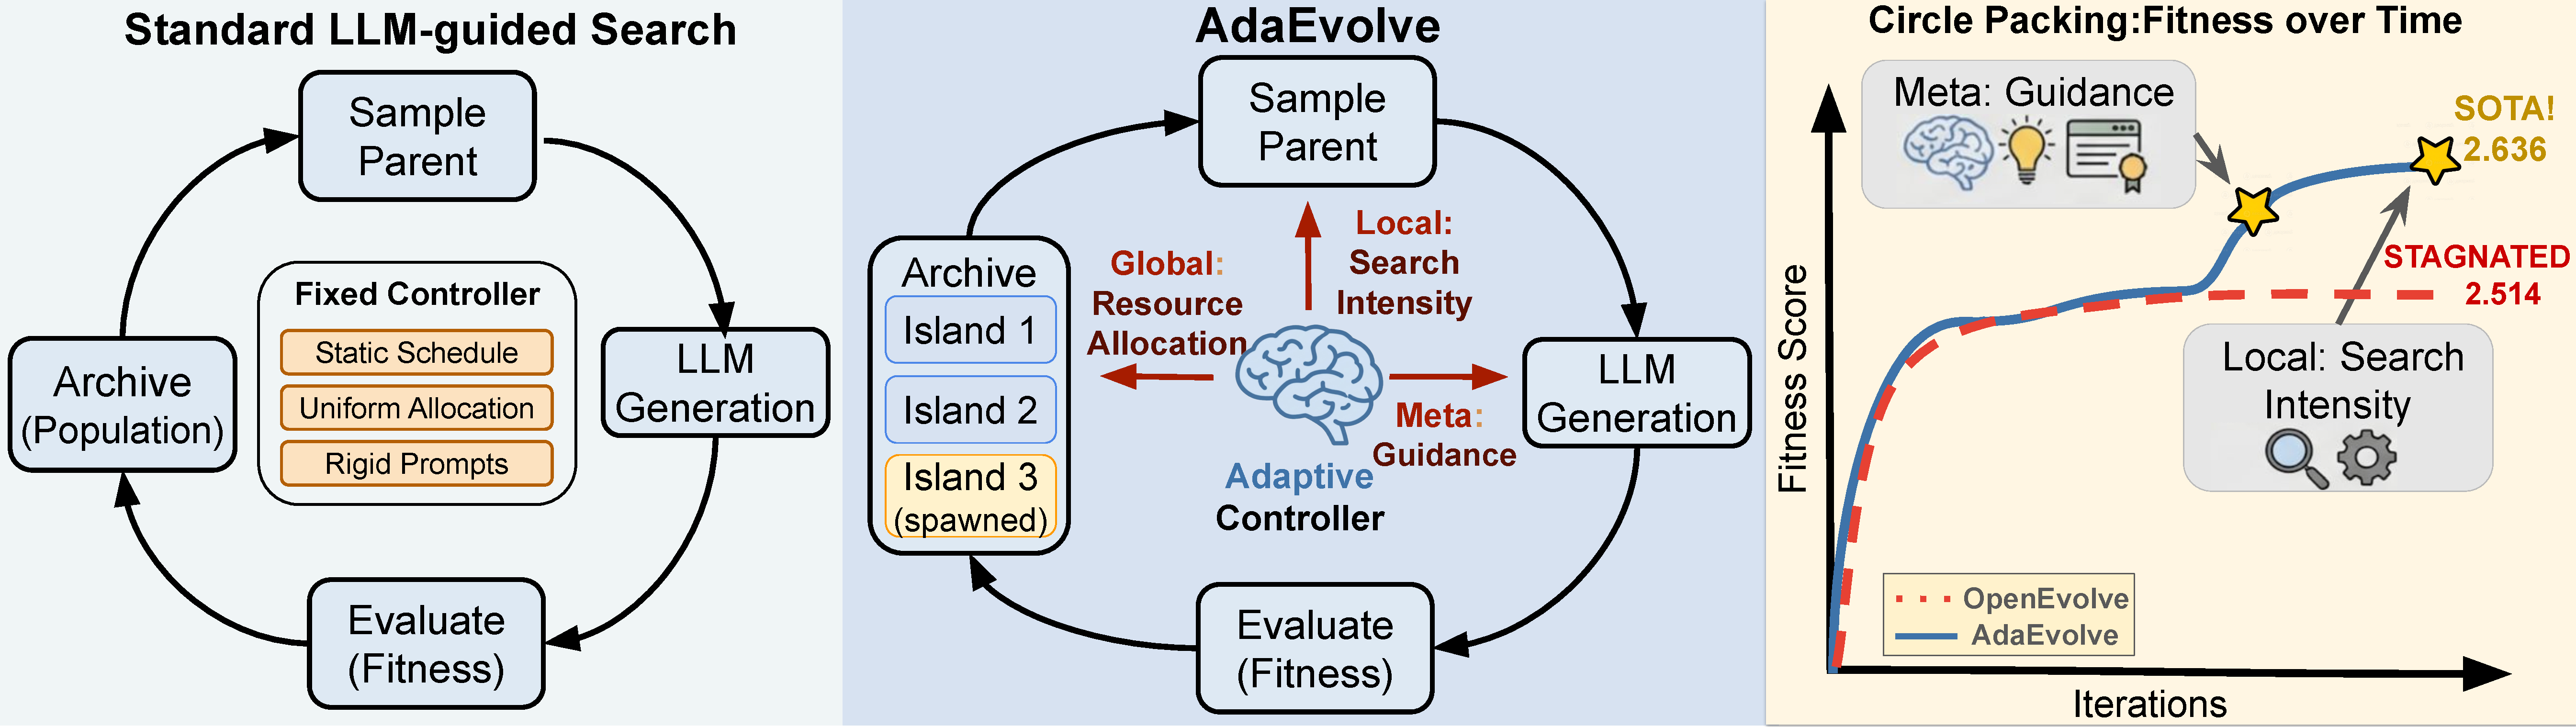
\includegraphics[width=0.96\textwidth]{figs/adaevolve_overview.pdf}
    \caption{\small AdaEvolve adapts search intensity, resource
             allocation, and meta-level guidance from a shared
             improvement signal. Figure from Cemri et al.\ (2025).}
  \end{figure}
\end{posterblock}

\begin{posterblock}{Optimizations}
  \heading{1.\enspace $K$-Batched Candidates per Iteration}
  One prompt, $K$ parallel calls with byte-identical prefixes.
  The first call prefills the KV cache; the other $K{-}1$ inherit it
  with \textbf{zero GPU prefill work}. Temperature is varied per call.

  \vspace{0.4em}
  \heading{2.\enspace Speculative Iteration Pipelining}
  Fire iteration $t{+}1$'s LLM calls \emph{during} iteration $t$'s
  CPU evaluation on a predicted prompt. A correct prediction hides
  an entire GPU prefill behind evaluation latency.

  \vspace{0.4em}
  \heading{3.\enspace GPU-Pressure Gating}
  Read \texttt{vllm:num\_requests\_running} from \texttt{/metrics};
  skip speculation when running\,/\,\texttt{max-num-seqs} $> 0.5$
  to avoid stealing slots under high load.

  \vspace{0.4em}
  \heading{4.\enspace Multi-Problem Orchestrator}
  $N$ problems share one vLLM endpoint. The static system-message
  prefix amortizes across all $N$ problems, boosting aggregate
  throughput on a single GPU.
\end{posterblock}

\begin{posterblock}{Experimental Setup}
  \begin{itemize}\setlength\itemsep{2pt}
    \item One \textbf{H100 80\,GB}; vLLM 0.15.1, prefix caching on,
          \texttt{max-num-seqs 32}
    \item Model: \textbf{Qwen3-4B-Instruct-2507}
    \item Two SkyDiscover benchmarks: \texttt{circle\_packing} and
          \texttt{signal\_processing}
    \item Up to $N{=}16$ concurrent problems; $K{=}8$ batched arms
  \end{itemize}
\end{posterblock}

\begin{posterblock}{Layered Speedup}
  \begin{figure}
    \centering
    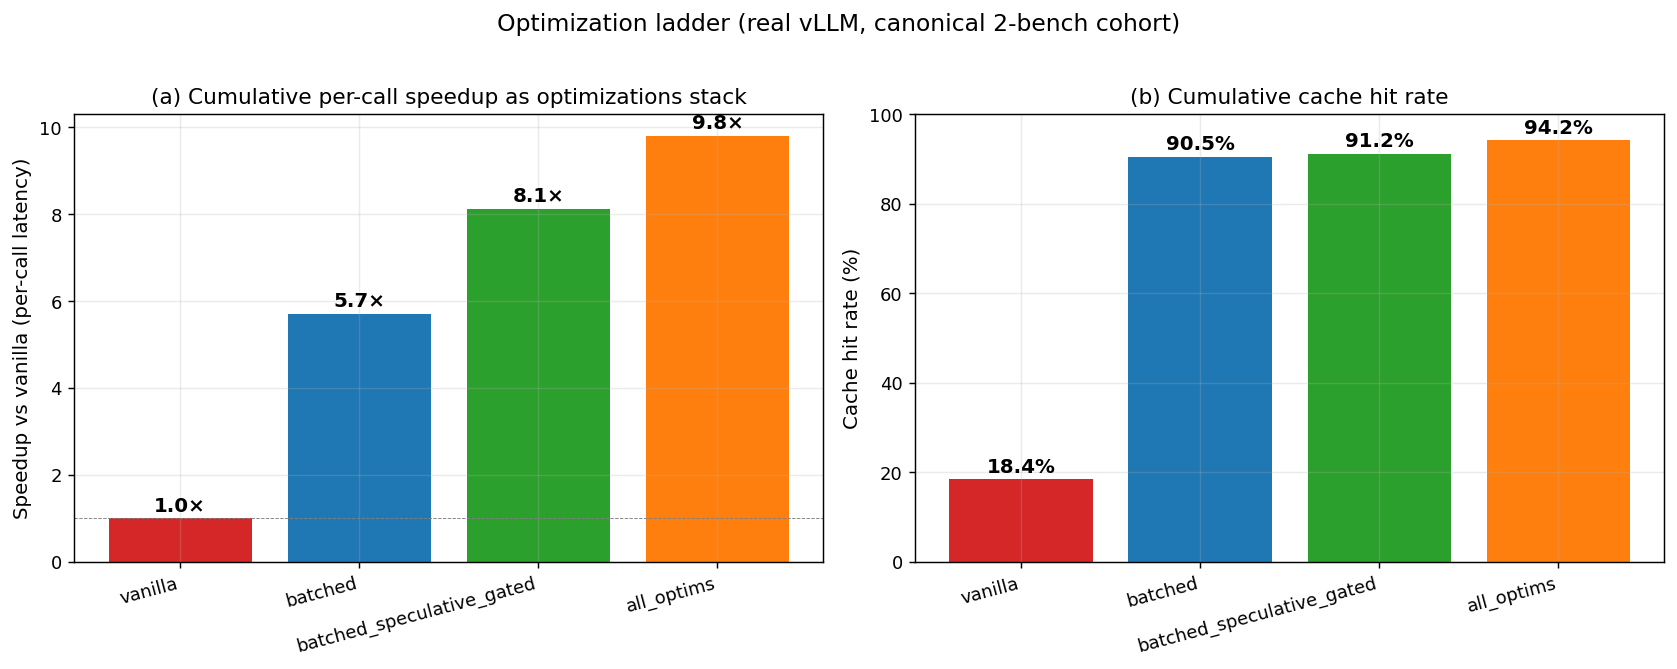
\includegraphics[width=0.96\textwidth]{figs/fig_optim_ladder.png}
    \caption{\small $K$-batching alone: 5.7$\times$ and 90\% hit rate.
             Gated speculation: 8.1$\times$.
             All optimizations: \textbf{9.8$\times$} and \textbf{94\%}.}
  \end{figure}
\end{posterblock}

\end{column}
\separatorcolumn

% ============================================================
%  COLUMN 3
% ============================================================
\begin{column}{\colwidth}

\begin{posterblock}{Headline Results}
  \begin{center}
  \renewcommand{\arraystretch}{1.2}
  \begin{tabular}{lcccc}
    \toprule
    \textbf{Configuration} & \textbf{Hit rate} & \textbf{Latency} &
    \textbf{Speedup} & \textbf{Score} \\
    \midrule
    Vanilla                    & 18.4\,\% & 6.30\,s & 1.0$\times$ & 0.364 \\
    Batched                    & 90.5\,\% & 1.10\,s & 5.7$\times$ & 0.548 \\
    Batched + spec.\ gated     & 91.2\,\% & 0.77\,s & 8.1$\times$ & 0.569 \\
    \textbf{All optimizations} & \textbf{94.2\,\%} & \textbf{0.64\,s}
                               & \textbf{9.8$\times$} & \textbf{0.604} \\
    \bottomrule
  \end{tabular}
  \end{center}
  \vspace{0.2em}
  \small Two benchmarks, $N{=}3$ iterations, $K{=}8$ arms, one H100.
  Hit rate 18\%~$\to$~94\%; latency drops 9.8$\times$.
\end{posterblock}

\begin{posterblock}{Multi-Problem Scaling}
  \vspace{2pt}
  \noindent
  \begin{minipage}[c]{0.55\linewidth}
    \centering
    \includegraphics[width=\linewidth, height=7.5cm, keepaspectratio]%
      {figs/fig_scaling_sweep.png}\\[3pt]
    {\scriptsize\textit{Figure:} Throughput (calls/s) vs.\ concurrent problems $N$.}
  \end{minipage}%
  \hfill
  \begin{minipage}[c]{0.41\linewidth}
    \small
    At $N{=}8$, batched delivers \textbf{37\% more candidates per
    second} than vanilla on the same GPU.\par\vspace{5pt}
    Speculation wins at low $N$ but \textbf{regresses at $N{=}8$}
    (wasted speculative compute steals scheduler slots).\par\vspace{5pt}
    The \textbf{GPU-pressure gate} recovers throughput at moderate
    concurrency with no algorithm changes.
  \end{minipage}
\end{posterblock}

\begin{posterblock}{Long-Run Quality}
  \centering
  \includegraphics[width=0.96\colwidth, height=11.5cm, keepaspectratio]%
    {figs/fig_long_run.png}\\[4pt]
  {\small\textit{Figure:} Vanilla at $K{=}1$ does not improve past
   the seed. Full stack at $N{=}16$ reaches \textbf{0.816}
   (AlphaEvolve target $=1.000$). Cache hit stays $\sim$95\%
   throughout.}
\end{posterblock}

\begin{posteralert}{Conclusions}
  \begin{itemize}\setlength\itemsep{3pt}
    \item \textbf{Root cause:} vLLM's chained block-hash breaks each
          iteration because the parent program mutates mid-prompt.
          Batching $K$ calls under one parent fixes this.
    \item \textbf{9.8$\times$ per-call speedup;} cache hit rate
          18\%~$\to$~94\% with all optimizations.
    \item \textbf{Quality improves too:} \texttt{circle\_packing}
          score 0.36~$\to$~0.82 after 16 iterations — more compute
          in the same wall time enables more exploration.
    \item \textbf{Gating matters at scale:} ungated speculation hurts
          at $N{=}8$; the pressure gate recovers throughput at
          moderate concurrency.
    \item \textbf{Future work:} async speculation gate at high $N$;
          multi-seed quality study; GRPO-in-the-loop.
  \end{itemize}
\end{posteralert}

\end{column}
\separatorcolumn
\end{columns}
\end{frame}
\end{document}